\documentclass[12pt]{report}
\usepackage[utf8]{inputenc}
\usepackage[russian]{babel}
%\usepackage[14pt]{extsizes}
\usepackage{listings}
\usepackage{graphicx}
\usepackage{amsmath,amsfonts,amssymb,amsthm,mathtools} 
\usepackage{pgfplots}
\usepackage{filecontents}
\usepackage{float}
\usepackage{indentfirst}
\usepackage{eucal}
\usepackage{enumitem}
%s\documentclass[openany]{book}
\frenchspacing

\usepackage{indentfirst} % Красная строка

\usetikzlibrary{datavisualization}
\usetikzlibrary{datavisualization.formats.functions}

\usepackage{amsmath}


% Для листинга кода:
\lstset{ %
	language=c,                 % выбор языка для подсветки (здесь это С)
	basicstyle=\small\sffamily, % размер и начертание шрифта для подсветки кода
	numbers=left,               % где поставить нумерацию строк (слева\справа)
	numberstyle=\tiny,           % размер шрифта для номеров строк
	stepnumber=1,                   % размер шага между двумя номерами строк
	numbersep=5pt,                % как далеко отстоят номера строк от подсвечиваемого кода
	showspaces=false,            % показывать или нет пробелы специальными отступами
	showstringspaces=false,      % показывать или нет пробелы в строках
	showtabs=false,             % показывать или нет табуляцию в строках
	frame=single,              % рисовать рамку вокруг кода
	tabsize=2,                 % размер табуляции по умолчанию равен 2 пробелам
	captionpos=t,              % позиция заголовка вверху [t] или внизу [b] 
	breaklines=true,           % автоматически переносить строки (да\нет)
	breakatwhitespace=false, % переносить строки только если есть пробел
	escapeinside={\#*}{*)}   % если нужно добавить комментарии в коде
}


\usepackage[left=2cm,right=2cm, top=2cm,bottom=2cm,bindingoffset=0cm]{geometry}
% Для измененных титулов глав:
\usepackage{titlesec, blindtext, color} % подключаем нужные пакеты
\definecolor{gray75}{gray}{0.25} % определяем цвет
\newcommand{\hsp}{\hspace{20pt}} % длина линии в 20pt
% titleformat определяет стиль
\titleformat{\chapter}[hang]{\Huge\bfseries}{\thechapter\hsp\textcolor{gray75}{|}\hsp}{0pt}{\Huge\bfseries}


% plot
\usepackage{pgfplots}
\usepackage{filecontents}
\usetikzlibrary{datavisualization}
\usetikzlibrary{datavisualization.formats.functions}

\begin{document}

\thispagestyle{empty}
\begin{titlepage}

\noindent \begin{minipage}{0.15\textwidth}
	
\includegraphics[width=\linewidth]{img/b_logo}
	\end{minipage}
	\noindent\begin{minipage}{0.9\textwidth}\centering
		\textbf{Министерство науки и высшего образования Российской Федерации}\\
		\textbf{Федеральное государственное бюджетное образовательное учреждение высшего образования}\\
		\textbf{~~~«Московский государственный технический университет имени Н.Э.~Баумана}\\
		\textbf{(национальный исследовательский университет)»}\\
		\textbf{(МГТУ им. Н.Э.~Баумана)}
	\end{minipage}
	
	\noindent\rule{18cm}{3pt}
	\newline\newline
	\noindent ФАКУЛЬТЕТ $\underline{\text{~~~~~~~~~~~~~~~~~~~«Информатика и системы управления»~~~~~~~~~~~~~~}}$ \newline\newline
	\noindent КАФЕДРА $\underline{\text{«Программное обеспечение ЭВМ и информационные технологии»}}$\newline\newline\newline\newline\newline
	
	\begin{center}
		\noindent\begin{minipage}{1.1\textwidth}\centering
			\Large\textbf{  Отчет по практике}\newline
			\textbf{Организация и проведение салона}
			\textbf{<<Шаг в будущее>>}\newline\newline
		\end{minipage}
	\end{center}
	
	

	\noindent\textbf{Студент} $\underline{\text{~~~~~~~~~~~~~~~~~~~~~~~~~~~~~~~~Костев Д.И.~~~~~~~~~~~~~~~~~~~~~~~~~~~~~~~~~~~~~~~~~~~~~~~~~~~~~~~~~~~~~~}}$\newline\newline
	\noindent\textbf{Группа} $\underline{\text{~~~~~~~~~~~~~~~~~~~~~~~~~~~~~~~~~~~~ИУ7-61Б~~~~~~~~~~~~~~~~~~~~~~~~~~~~~~~~~~~~~~~~~~~~~~~~~~~~~~~~~~~~~~~~~}}$\newline\newline
	\noindent\textbf{Тип практики} $\underline{\text{~~~~~~~~~~~~~~~~~~~~~~~~~Производственная~~~~~~~~~~~~~~~~~~~~~~~~~~~~~~~~~~~~~~~~~~~~~~~~~~~~~}}$\newline\newline
	\noindent\textbf{Название предприятия} $\underline{\text{~~~~~~~~~~~~МГТУ им. Н. Э. Баумана, каф. ИУ7~~~~~~~~~~~~~~~~~~~~~~~~~~~}}$\newline\newline\newline\newline
	
	
	\noindent\begin{tabular}{lcc}
		Студент: ~~~~~~~~~~~~~~~~~~~~~~~~~~~~~~~~~~~~~~~~~~~~~~~~~~~~~~~~ & $\underline{\text{~~~~~~~~~~~~~~~~}}$ & $\underline{\text{~~Костев Д.И.~~}}$     \\
            & \footnotesize подпись, дата           & \footnotesize Фамилия, И.О.              \\
		%& &  \\

		Руководитель практики от МГТУ им. Н.Э.Баумана:                                                    &  $\underline{\text{~~~~~~~~~~~~~~~~}}$ & $\underline{\text{~~~~Толпинская Н.Б.~~~}}$ \\
            & \footnotesize подпись, дата           & \footnotesize Фамилия, И.О.              \\
		%& &  \\
            Руководитель практики от предприятия:                                                    & $\underline{\text{~~~~~~~~~~~~~~~~}}$ & $\underline{\text{~~~~Волкова Л.Л.~~~}}$ \\
            & \footnotesize подпись, дата           & \footnotesize Фамилия, И. О.             \\
	\end{tabular}


\begin{center}
	\vfill
	Москва~---~\the\year
	~г.
\end{center}

\end{titlepage}

\tableofcontents

\chapter*{Введение}

Ежегодно кафедра ИУ7 проводит конкурс <<Шаг в будущее>> для абитуриентов.
В 2022 году данное мероприятие было проведено 26 марта. 

Целью практики являлась организация и проведения данного конкурса.

В рамках выполнения практики необходимо решить следующие задачи.

\begin{enumerate}
	\item Установить необходимое ПО.
	% \item Составить схему рассадки участников и подготовить необходимые документы для проведения конкурса.
	% \item Информирование абитуриентов, которые участвуют в конкурсе, о правилах проведения. 
	\item Изучение и оценка работ участников.
	\item Составление рецензий.
	% \item Подготовка аудитории к проведению конкурса.
	% \item Организация работы студенческого жюри.
	% \item Проверка работоспособности ПО после окончания конкурса.
	% \item Вручение призов.
\end{enumerate}

\chapter{Основная часть}

\section{Установка необходимого ПО}

Для установки необходимого ПО нужно было знать, какое ПО нужно каждому участнику.
Поэтому до проведения конкурса был произведен обзвон каждого участника конкурса с целью 
уточнения необходимого им ПО. Для тех участников, которым необходим был стационарный компьютер
для презентации работы было установлено запрошенное ПО.
Список языков программирования, необходимых участникам:

\begin{itemize}
	\item Python3;
	\item C\#;
	\item .NET framework;
	\item Pascal ABC.NET;
	\item C++;
	\item Swift 5.
\end{itemize}

Также для проведения конкурса некоторым участникам необходим был интернет.
До проведения конкурса каждого участника спрашивали о необходимости в использовании интернета.
Если участнику нужен был интернет ему предлагалось авторизоваться через бауманскую сеть для получения интернета.

\section{Составление схемы рассадки участников и подготовление необходимых документов для проведения конкурса}

После получения информации от участников конкурса о том, нужен ли им стационарный компьютер или нет
была составлена рассадка, которая учитывала наличие собственного ноутбука. 
Были проверены стационарные компьютеры на работоспособность.

% Рассадка представлена на рис. \ref{ref:1}

% \begin{figure}[ht!]	
% 	\centering{
% 		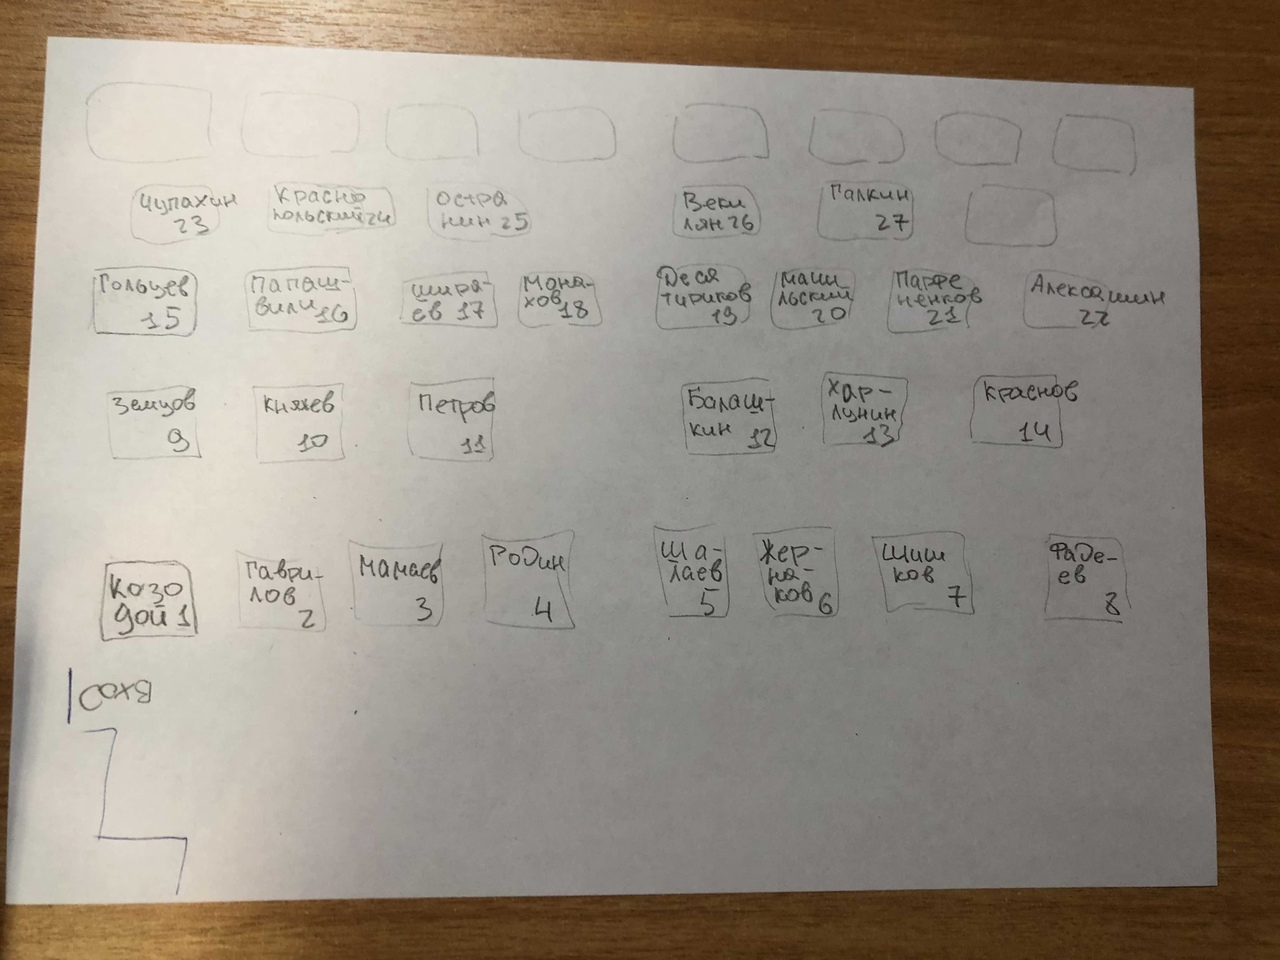
\includegraphics[width=0.9\textwidth]{img/img1.jpg}
% 		\caption{Рассадка участников конкурса}
% 		\label{ref:1}}
% \end{figure}

Для каждого участника конкурса был сделан бумажный указатель, идентифицирующий его проект, чтобы 
в дальнейшем каждый участник конкурса смог в точности знать свой стол. 

Также были распечатаны рецензии, которые заполнялись после проведения конкурса, 
листы с данными о каждом участнике, в котором они должны были расписываться за присутствие на конкурсе. 
Также были подготовлены именные бейджи для студенческого жюри и для членов экспертной комиссии. 

\section{Информирование абитуриентов, которые участвуют в конкурсе, о правилах проведения}

Предварительно нужно было информировать всех участников о дате проведения конкурса 
и о правилах. Организаторы имели список участников и их номера. 
Иногда номера были недоступны, тогда организаторы пытались найти участника в соц. сетях.

\chapter{Изучение работы участника}

\section{Сведения о участнике и его работе}

При проведении конкурса студенческое жюри просматривали и оценивали работы участников.
Мною была проанализирована одна из работ.

Работа была сделана Соколовым Дмитрием Максимовичем, учеником 11-В класса школа №1580.
Тема рассматриваемой работы: <<Анализатор речи для проверки соответствия слов тексту.
Компьютерное приложение «Lyrics Listener»>> На рис. \ref{ref:2} показана работа одного из участника конкурса.

\begin{figure}[ht!]	
	\centering{
		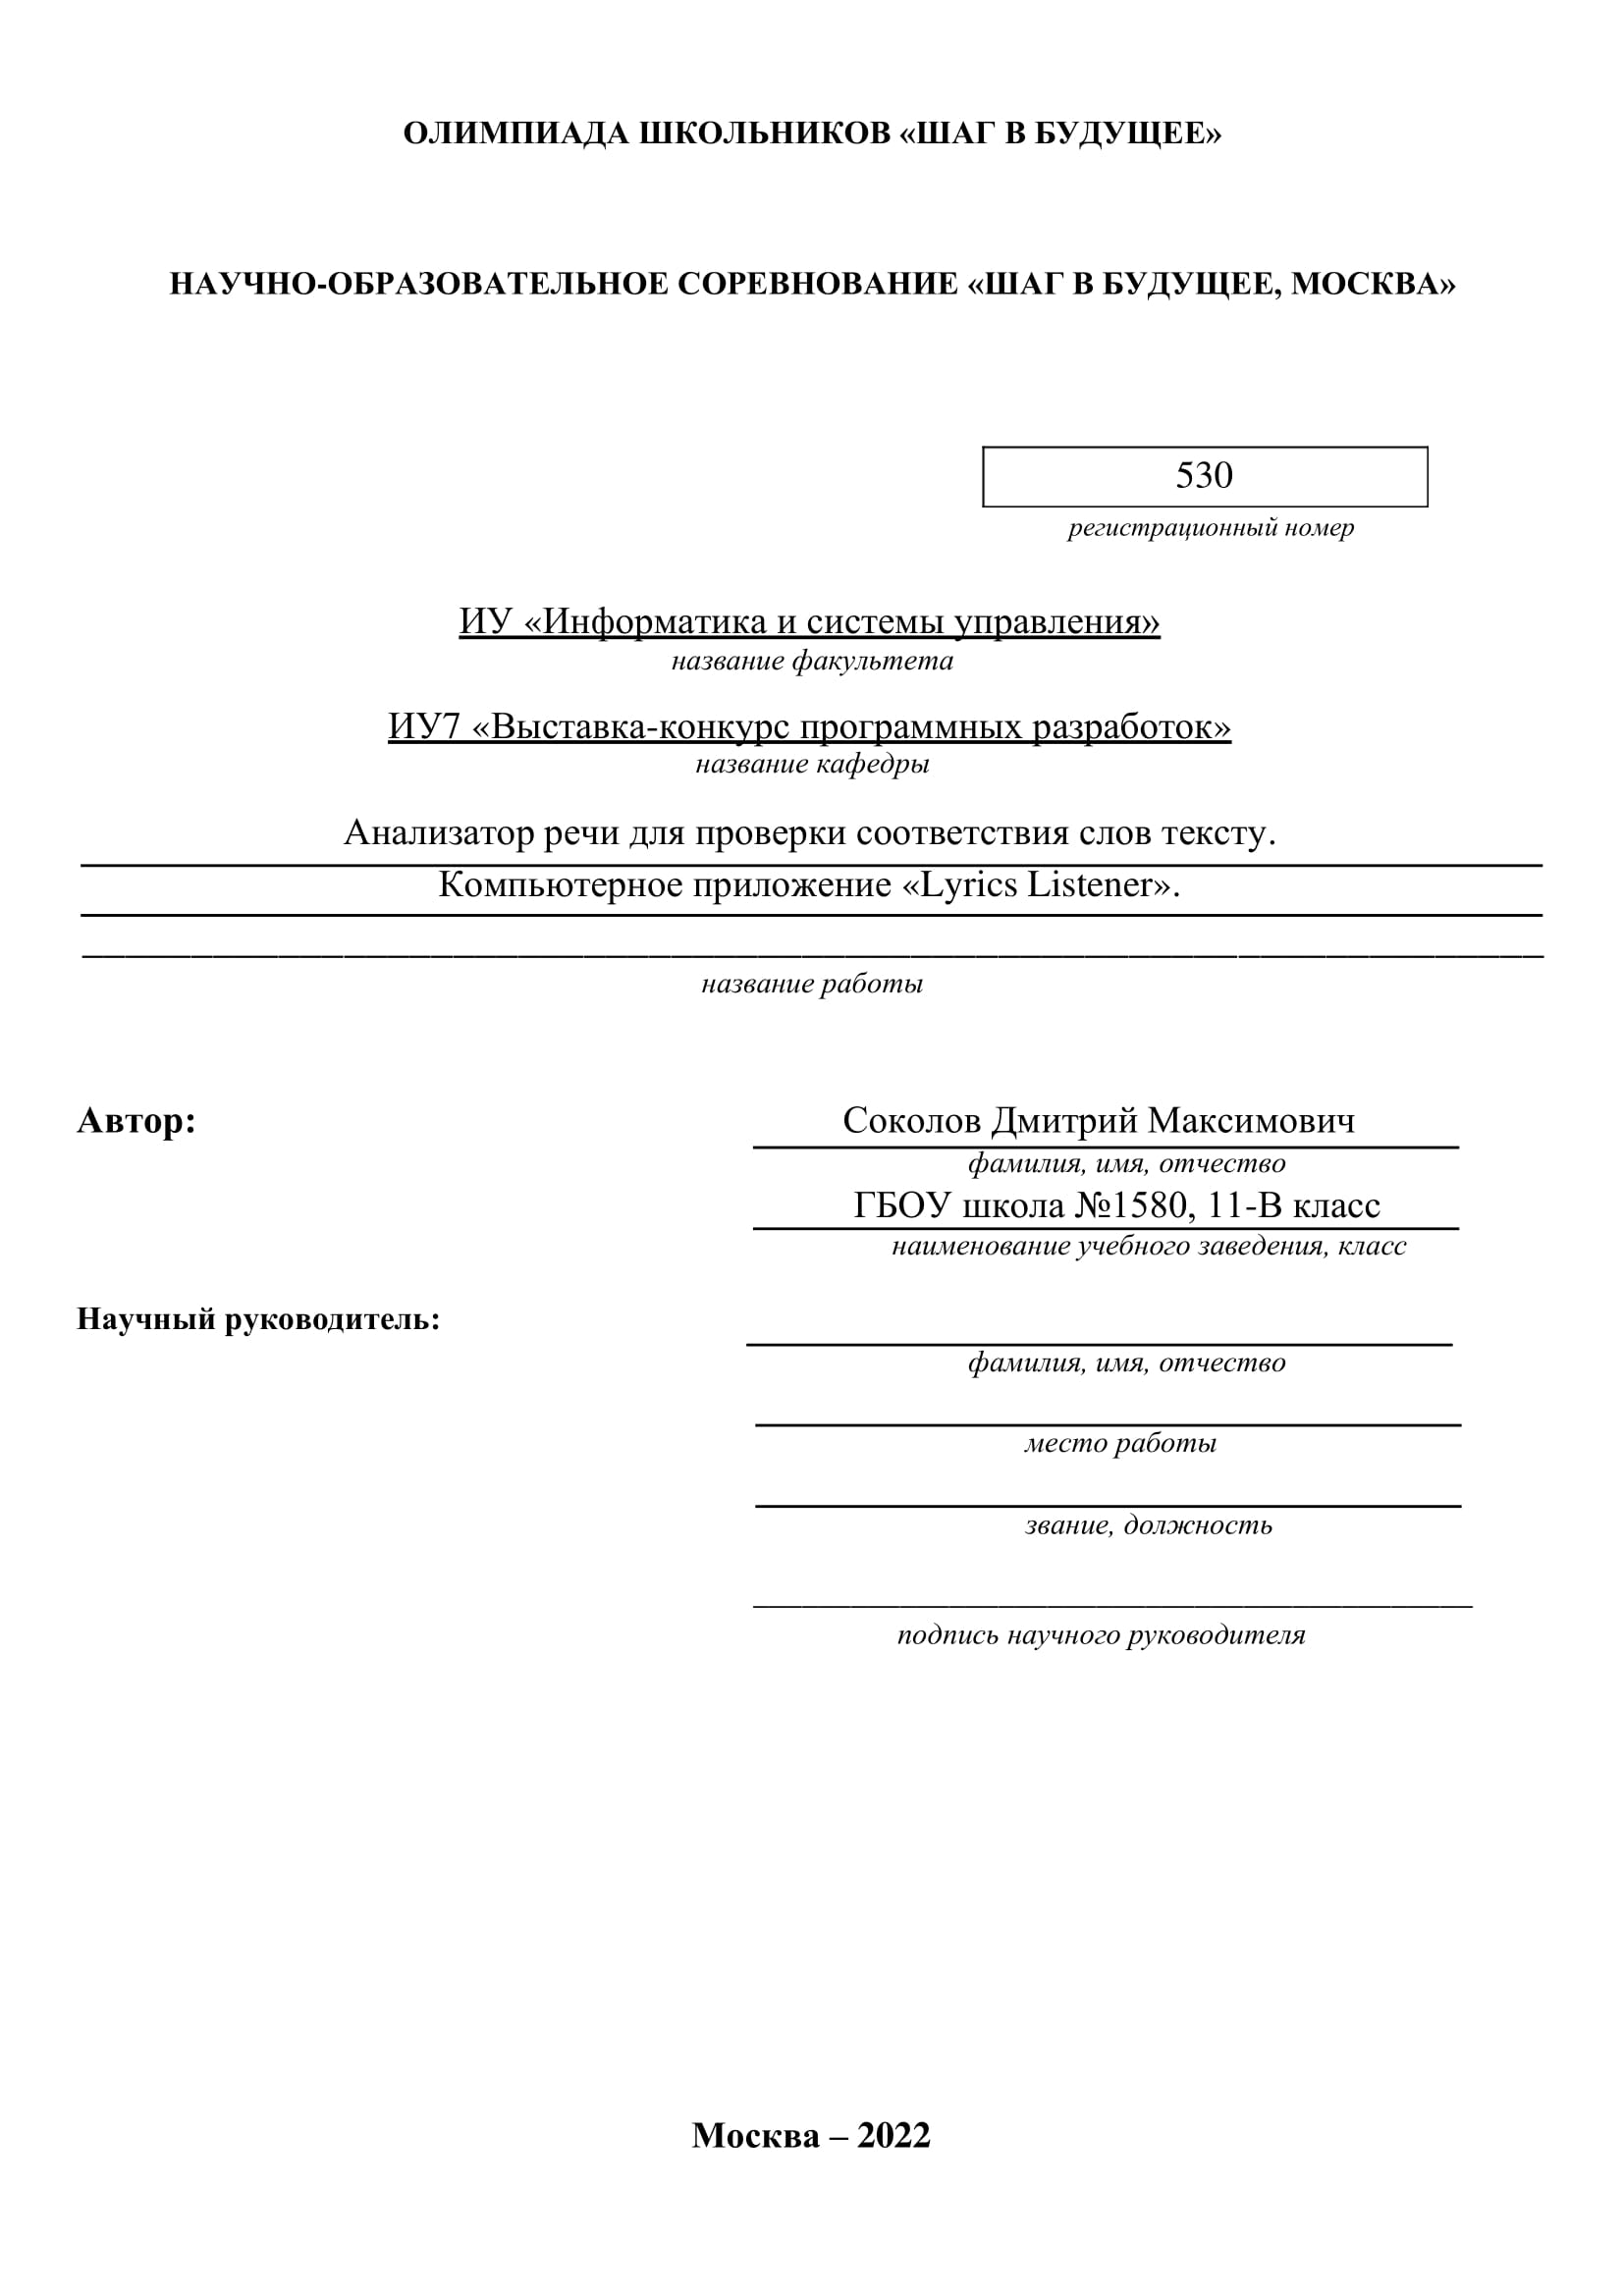
\includegraphics[width=0.8\textwidth]{img/img2.jpg}
		\caption{Работа одного из участника конкурса}
		\label{ref:2}}
\end{figure}
\section{Цель работы}

Работа данного участника была создана с целью внедрения в учебный процесс
собственных разрабатываемых технологий для автоматизации учебного процесса.
Было решено разработать компьютерное приложение для анализа текстов и записанного голоса на соответствие слов.

\section{Возможности предоставленного ПО}

В версии, которая была предоставлена на показ с помощью компьютерного приложения, можно было
загрузить текст стиха и файл записи голоса.

Участник проекта предусматривал дальнейшую работу над проектом,
как дальнейшее исполнение плана, где глобальная миссия -- добавить функцию записи голоса прямо в приложение.

\section{Поставленные задачи}

Участник поставил перед собой задачу сделать компьютерное приложение для сравнения текста, сказанного голосом и напечатанного. 

Участник провел опрос сверстников и проанализировал собранные материалы после чего 
выявил функциональность первой необходимости — это заучивание каких-либо текстов и проверка выученного.

\section{Оценка актуальности темы}

Участник заявил, что <<Согласно опросам, подобных технологий нет на рынке приложений>>

Я считаю, что поставленная им задача не актуальна в учебном процессе, но может быть хорошо внедрена в иной сфере деятельности. Подобное решение лучше могло бы использоваться для изучения иностранных языков. Например, проверка правильности произношения, таким образом человек сможет корректировать свою речь без участия других людей(носителей речи, преподавателей языка).

\section{Архитектура приложения}

Для проекта был выбран классическая паттерн MVP(Model Veiw Presenter). \ref{ref:3}.

\begin{figure}[ht!]	
	\centering{
		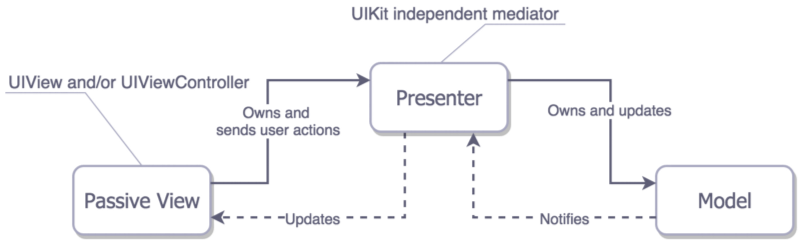
\includegraphics[width=0.9\textwidth]{img/img3.png}
		\caption{Патерен MVP}
		\label{ref:3}}
\end{figure}

Данная архитектура делит проект на визуальную часть (VIEW) с представителем для нее (PRESENTER) и модель (MODEL).

Ниже представлен список всех технологий использованных в проекте.
\begin{enumerate}
    \item Python 3.9
    \item GNU C++ 11.1.0
    \item PyQT5
    \item threading
    \item sys
    \item pymystem3
    \item abc
    \item vosk
    \item queue
    \item json
    \item sounddevice
    \item pybind11 (для C++ и Python)
    \item distuils.core
    \item string
    \item vector
    \item iterator
    \item algorithm
    \item iostream
    \item sstream
    \item set
\end{enumerate}

\section{Заключение}

Поставленная участником цель была достигнута:

\begin{itemize}
	\item разработано компьютерное приложение для анализа текстов и записанного голоса на соответствие слов.
\end{itemize}

\chapter{Окончание конкурса}

\section{Вручение призов}

По окончанию проведения конкурса <<Шаг в будущее>>
было произведено голосование студенческого жюри и членов экспертной комиссии, 
по итогом которого было назначено 3 победителя. 

После чего всех участников пригласили на церемонию вручения призов, где трем победителям вручили призы.

\section{Составление рецензий}

Организаторы получили бланки для оценивания выступления и работы каждого участника.
Бланк состоит из двух частей -- оценки работы и резюме рецензента. 
В оценочной части необходимо поставить оценку от 0 до 4 по следующим критериям:

\begin{itemize}
	\item структура и оформление работы (качество оформления, грамотность содержания, ошибки, опечатки, выводы);
	\item логика изложения, оригинальность мышления, творческий подход;
	\item используемые методы (причины использования данных методов, эффективность, точность и простота методов);
	\item оригинальность тематики проекта, проверка текста научно-исследовательской на наличие заимствования из открытых
	источников в сети Интернет и других источников, актуальность тематики работы;
	\item научное и практическое значение работы;
\end{itemize}

На рис. \ref{ref:9} показан пример заполнения рецензии

\begin{figure}[ht!]	
	\centering{
		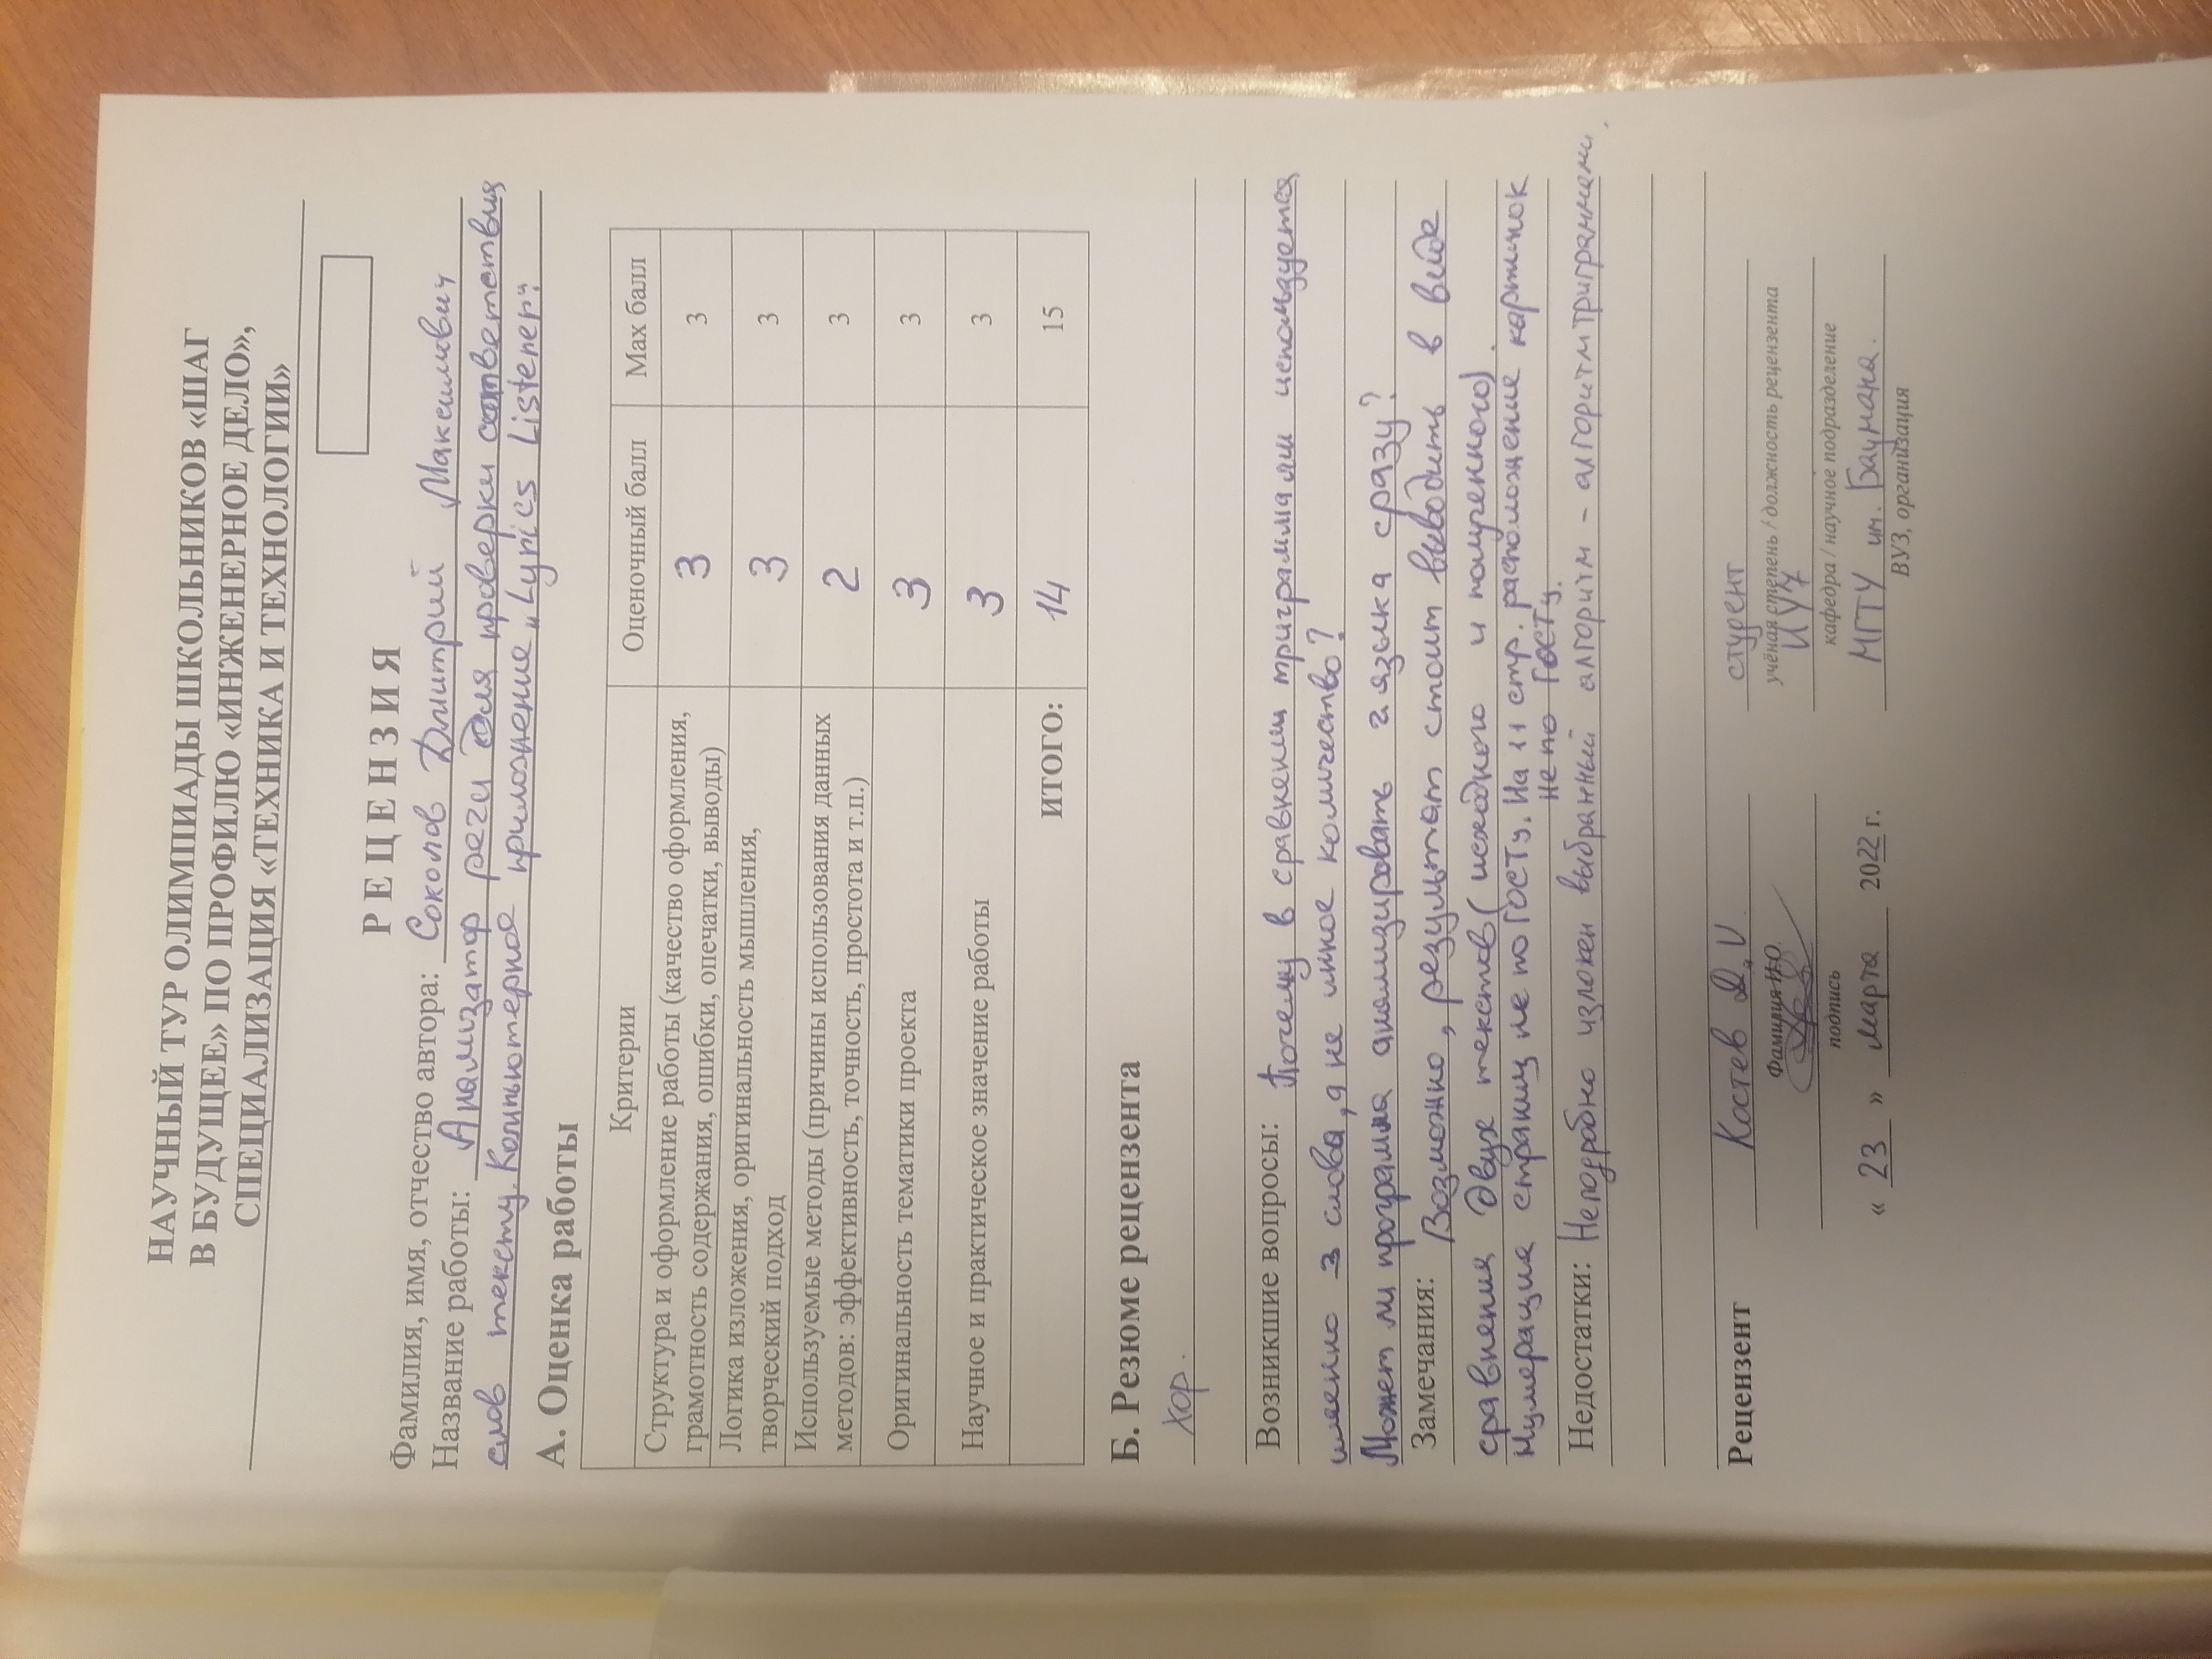
\includegraphics[width=1\textwidth, angle=-90]{img/img9.jpg}
		\caption{Пример заполнения рецензии студенческого жюри}
		\label{ref:9}}
\end{figure} 

\chapter{Заключение}

Была пройдена практика по проведению программного салона <<Шаг в будущее>>.
Был организован конкурс, в результате которого были определены победители конкурса.
Руководство кафедры ИУ7 объявило устную благодарность организаторам салона.

Были выполнены следующие задачи.

\begin{enumerate}
	\item Установлено необходимое ПО.
	% \item Составлена схема рассадки участников и подготовлены необходимые документы для проведения конкурса.
	% \item Информированы абитуриенты, которые участвуют в конкурсе, о правилах проведения. 
	\item Изучена и оценена работа участника.
	\item Составлены рецензии.
	% \item Вручены призы.
\end{enumerate}


Цель, поставленная во время прохождения практики, была достигнута. 

\end{document}